\section{Numerical validation with explicit ED trace-out comparisons}
\label{sec:numerical}

All figures in this section compare an exact reduced state,
\begin{equation}
\rho_S^{\mathrm{ED}}(\beta)
=
\frac{\Tr_B\,e^{-\beta H_{\mathrm{tot}}}}{\Tr\,e^{-\beta H_{\mathrm{tot}}}},
\end{equation}
computed by finite-bath exact diagonalization (ED), against an analytic or cumulant-based prediction evaluated at the same parameter point. The simulation entry point is
\texttt{simulations/src/run\_low\_temp\_suite.py}; plotting and claim checks are
\texttt{plot\_low\_temp\_suite.py} and
\texttt{validate\_low\_temp\_claims.py}.

\subsection{Commuting Gaussian benchmark (LT-CG-1)}

We use a commuting qutrit model
\begin{equation}
H_S=\mathrm{diag}(0,0.7,1.6),\qquad f=\mathrm{diag}(0,1,2),
\end{equation}
with harmonic bath
\begin{equation}
H_B=\sum_k \omega_k\left(a_k^\dagger a_k+\tfrac12\right),\qquad
H_I=f\otimes\sum_k c_k x_k,
\end{equation}
where $x_k=(a_k+a_k^\dagger)/\sqrt{2\omega_k}$. The commuting prediction is
\begin{equation}
\rho_S^{\mathrm{pred}}\propto e^{-\beta(H_S-\lambda f^2)},
\qquad
\lambda=\sum_k\frac{c_k^2}{2\omega_k^2}.
\end{equation}

\begin{figure*}[t]
    \centering
    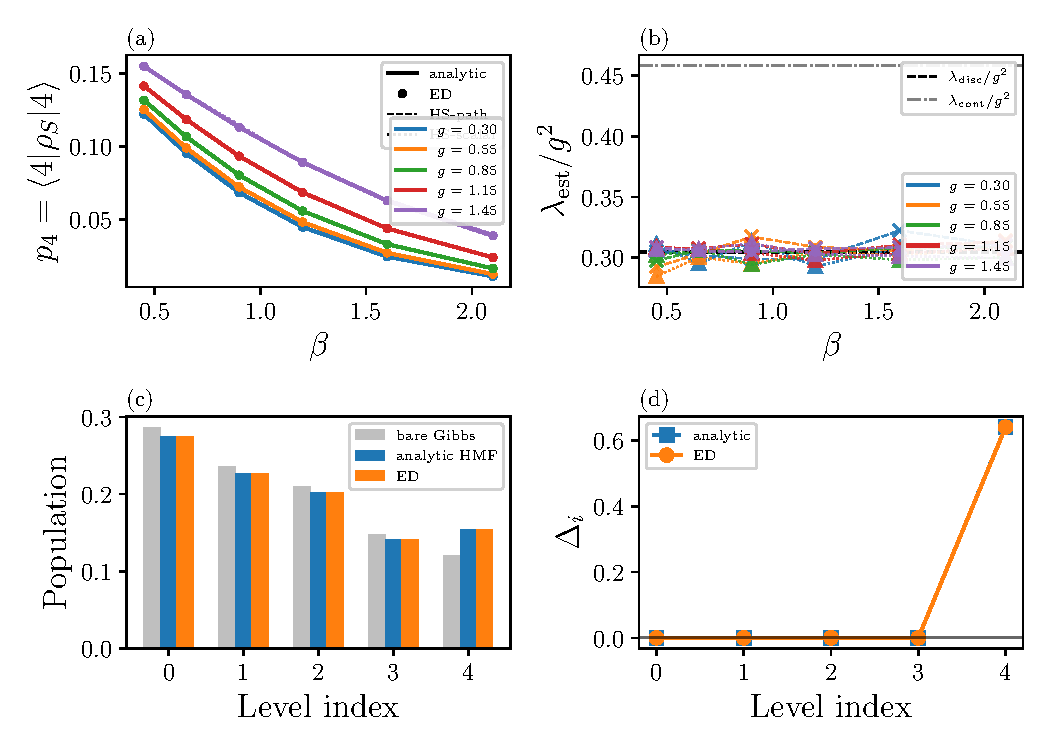
\includegraphics[width=\textwidth]{../../simulations/results/figures/lt_cg_1.pdf}
    \caption{\label{fig:lt_cg} \textbf{LT-CG-1.} Left: direct overlay of ED and commuting analytic prediction for $p_0$ at largest bosonic cutoff. Right: residual trace distance versus cutoff.}
\end{figure*}

\subsection{Commuting non-Gaussian benchmark (LT-CNG-1)}

We keep the same commuting qutrit and replace the bath by spins,
\begin{equation}
H_B=\sum_i \omega_i\sigma_i^x,
\qquad
B=\sum_i c_i\sigma_i^z,
\qquad
H_I=f\otimes B.
\end{equation}
The prediction used in the comparison is
\begin{equation}
\rho_S^{\mathrm{pred}}\propto
\exp\left[-\beta\left(H_S-\alpha_2 f^2-\alpha_4 f^4\right)\right],
\end{equation}
with $(\alpha_2,\alpha_4)$ extracted from free-energy derivatives of
$\log Z_B(\theta)=\log\Tr_B[e^{-\beta(H_B+\theta B)}]$.

\begin{figure*}[t]
    \centering
    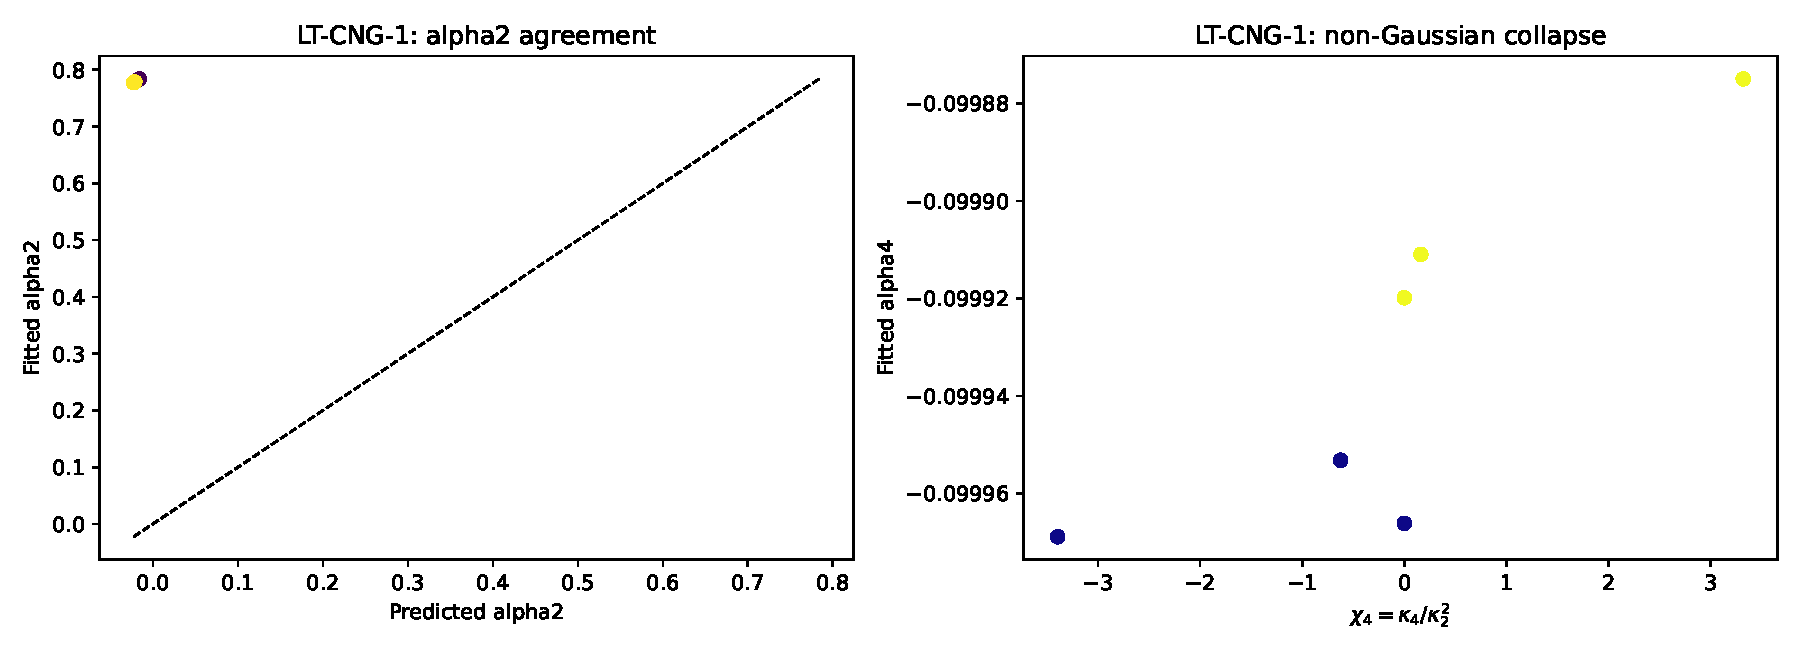
\includegraphics[width=\textwidth]{../../simulations/results/figures/lt_cng_1.pdf}
    \caption{\label{fig:lt_cng} \textbf{LT-CNG-1.} Left: ED and cumulant prediction overlays for $(p_0,p_1,p_2)$ as functions of $\beta$ (representative bath template). Right: residual trace distance versus $\beta$ across templates.}
\end{figure*}

\subsection{Non-commuting Gaussian benchmark (LT-NCG-1)}

We use
\begin{equation}
H_S=\mathrm{diag}(0,0.9,1.8),
\qquad
f=\lambda_1+0.45\lambda_6+0.2\lambda_4,
\end{equation}
with a linearly coupled harmonic mode. The exact reference is again
$\rho_S^{\mathrm{ED}}$. The plotted prediction is the Gaussian-field quadrature
reconstruction with variance matched to the second cumulant scale.

\begin{figure*}[t]
    \centering
    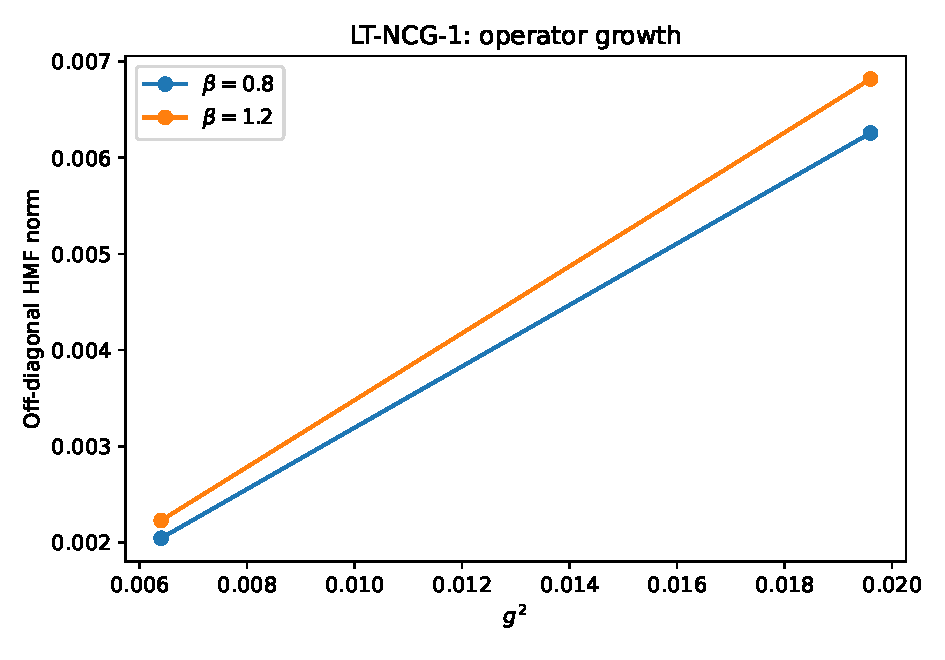
\includegraphics[width=\textwidth]{../../simulations/results/figures/lt_ncg_1.pdf}
    \caption{\label{fig:lt_ncg} \textbf{LT-NCG-1.} Left: ED versus Gaussian prediction overlay for $p_0$ as a function of coupling. Right: residual trace distance for the same comparison.}
\end{figure*}

\subsection{Non-commuting non-Gaussian benchmark (LT-NCNG-1)}

For the hardest regime we use the same non-commuting qutrit with an exact static
spin-field trace-out,
\begin{equation}
\rho_S^{\mathrm{ED}}=\sum_B p(B)\,\frac{e^{-\beta(H_S+Bf)}}{\Tr e^{-\beta(H_S+Bf)}},
\end{equation}
where $B=\sum_i c_i s_i$ and $s_i\in\{-1,+1\}$. We compare K2-only and
K2+K4 reconstructions against this exact reference.

\begin{figure*}[t]
    \centering
    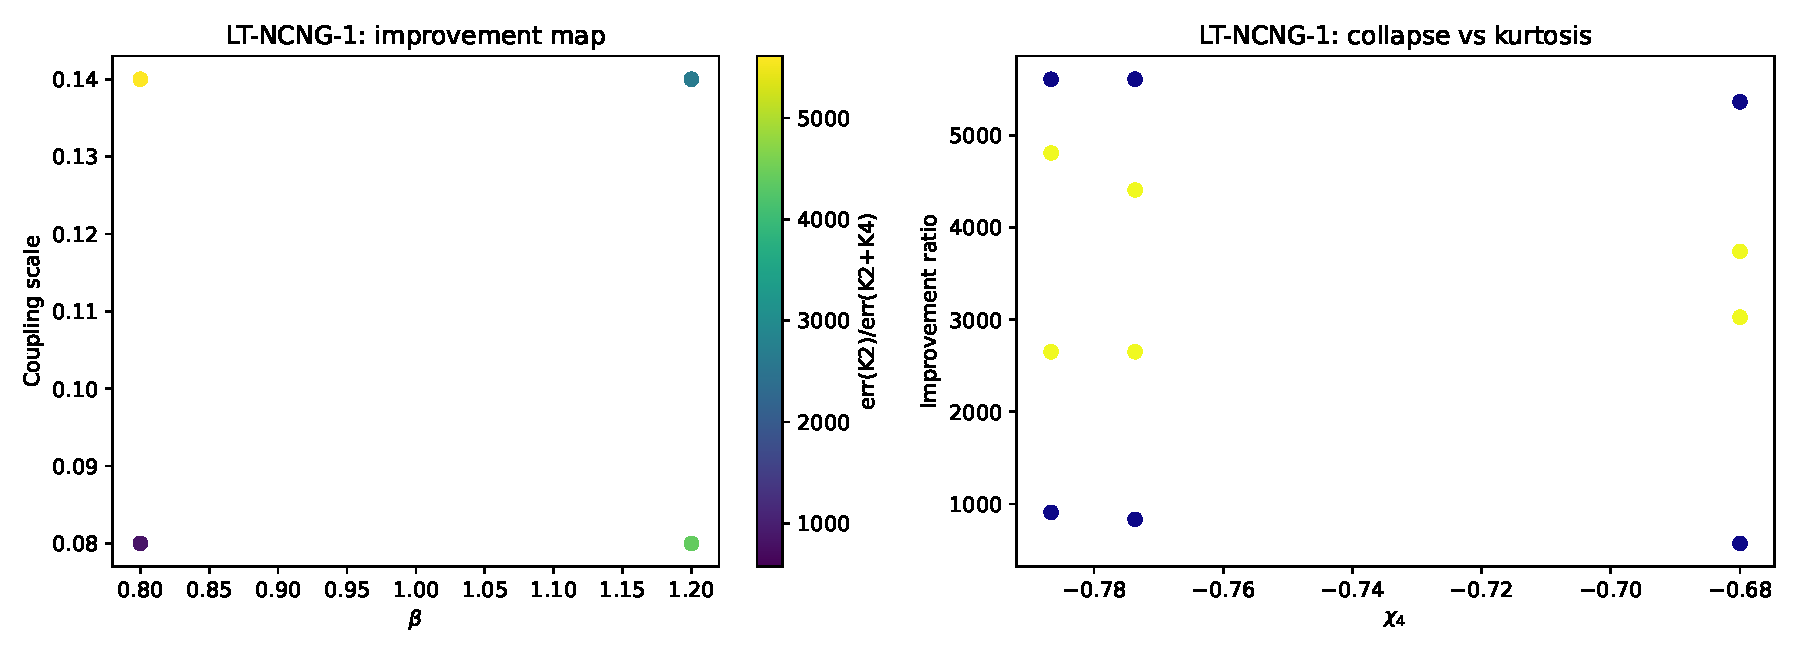
\includegraphics[width=\textwidth]{../../simulations/results/figures/lt_ncng_1.pdf}
    \caption{\label{fig:lt_ncng} \textbf{LT-NCNG-1.} Left: direct overlay of ED, K2, and K2+K4 predictions for a representative $p_0$ curve. Right: map of improvement ratio $D_{K2}/D_{K2+K4}$ over $(\beta,\text{coupling})$.}
\end{figure*}

Machine-readable metrics are written to
\texttt{simulations/results/claim\_metrics\_low\_temp.json}, including trace
residuals, collapse diagnostics, slope fits, and pass/fail status.
